% 
% Phantasia printable manual
% 
% This needs a lot of work yet.
% 
% If you're a human, skip to "\mainmatter" to skip over the preamble.
% 
\documentclass[10pt,twocolumn,openany,article]{memoir}

\ifdefined\ATARIAGESAVE
\setstocksize{9in}{6in}
\settrimmedsize{\stockheight}{\dimexpr 6in-15mm}{*}
\else
\setstocksize{11in}{8.5in}
\settrimmedsize{\stockheight}{\dimexpr 8.5in-15mm}{*}
\fi

\setlrmarginsandblock{.333333in}{.5in}{*}
\setulmarginsandblock{.75in}{.75in}{*}
\setheadfoot{.5in}{.5in}
\widowpenalty=10000
\clubpenalty=10000

\makeevenhead{plain}{\textit{Phantasia}}{}{}
\makeoddhead{plain}{}{}{\textit{Phantasia}}

\makeevenfoot{plain}{\thepage}{}{}
\makeoddfoot{plain}{}{}{\thepage}

\usepackage[utf8]{inputenc}
\usepackage{babel}
\usepackage{stfloats}
\usepackage{microtype}
\usepackage{graphicx}
\usepackage{pdfpages}
\tolerance=1
\emergencystretch=\maxdimen
% \usepackage{tgtermes}
\usepackage{hyperref}
\usepackage{xcolor}
\hypersetup{
  colorlinks,
  linkcolor={black},
  citecolor={blue!50!black},
  urlcolor={blue!80!black},
  pdftitle={Phantasia \ifdefined\DEMO{ Demo }\fi Manual},
  pdfsubject={Phantasia videogame for the Atari 7800},
  pdfauthor={Bruce-Robert Pocock}%,
  % pdfkeywords={Your PDF keywords}
}
\usepackage{caption}
\captionsetup{labelformat=empty}

\usepackage{tikz}

\newcommand\encircle[1]{%
  \tikz[baseline=(X.base)] 
  \node (X) [draw, shape=circle, inner sep=.25pt] {#1};}

\setlength{\columnsep}{.333333in}
%% \setlength\columnseprule{.5pt}

\usepackage{lettrine}
\usepackage[protrusion=true,expansion=true]{microtype}
\fontfamily{pnc}
\chapterstyle{komalike}

\checkandfixthelayout

\title{Phantasia \ifdefined\DEMO Demo \fi Player's Guide}
\author{Bruce-Robert Pocock}

% 
% 
% 
%%% BEGIN DOCUMENT
% 
% 
% 

\begin{document}

\frontmatter
\thispagestyle{empty}

\begin{tikzpicture}[overlay, remember picture]
  \node[anchor=north west, xshift=-4pt, yshift=4pt] 
  at (current page.north west)
  {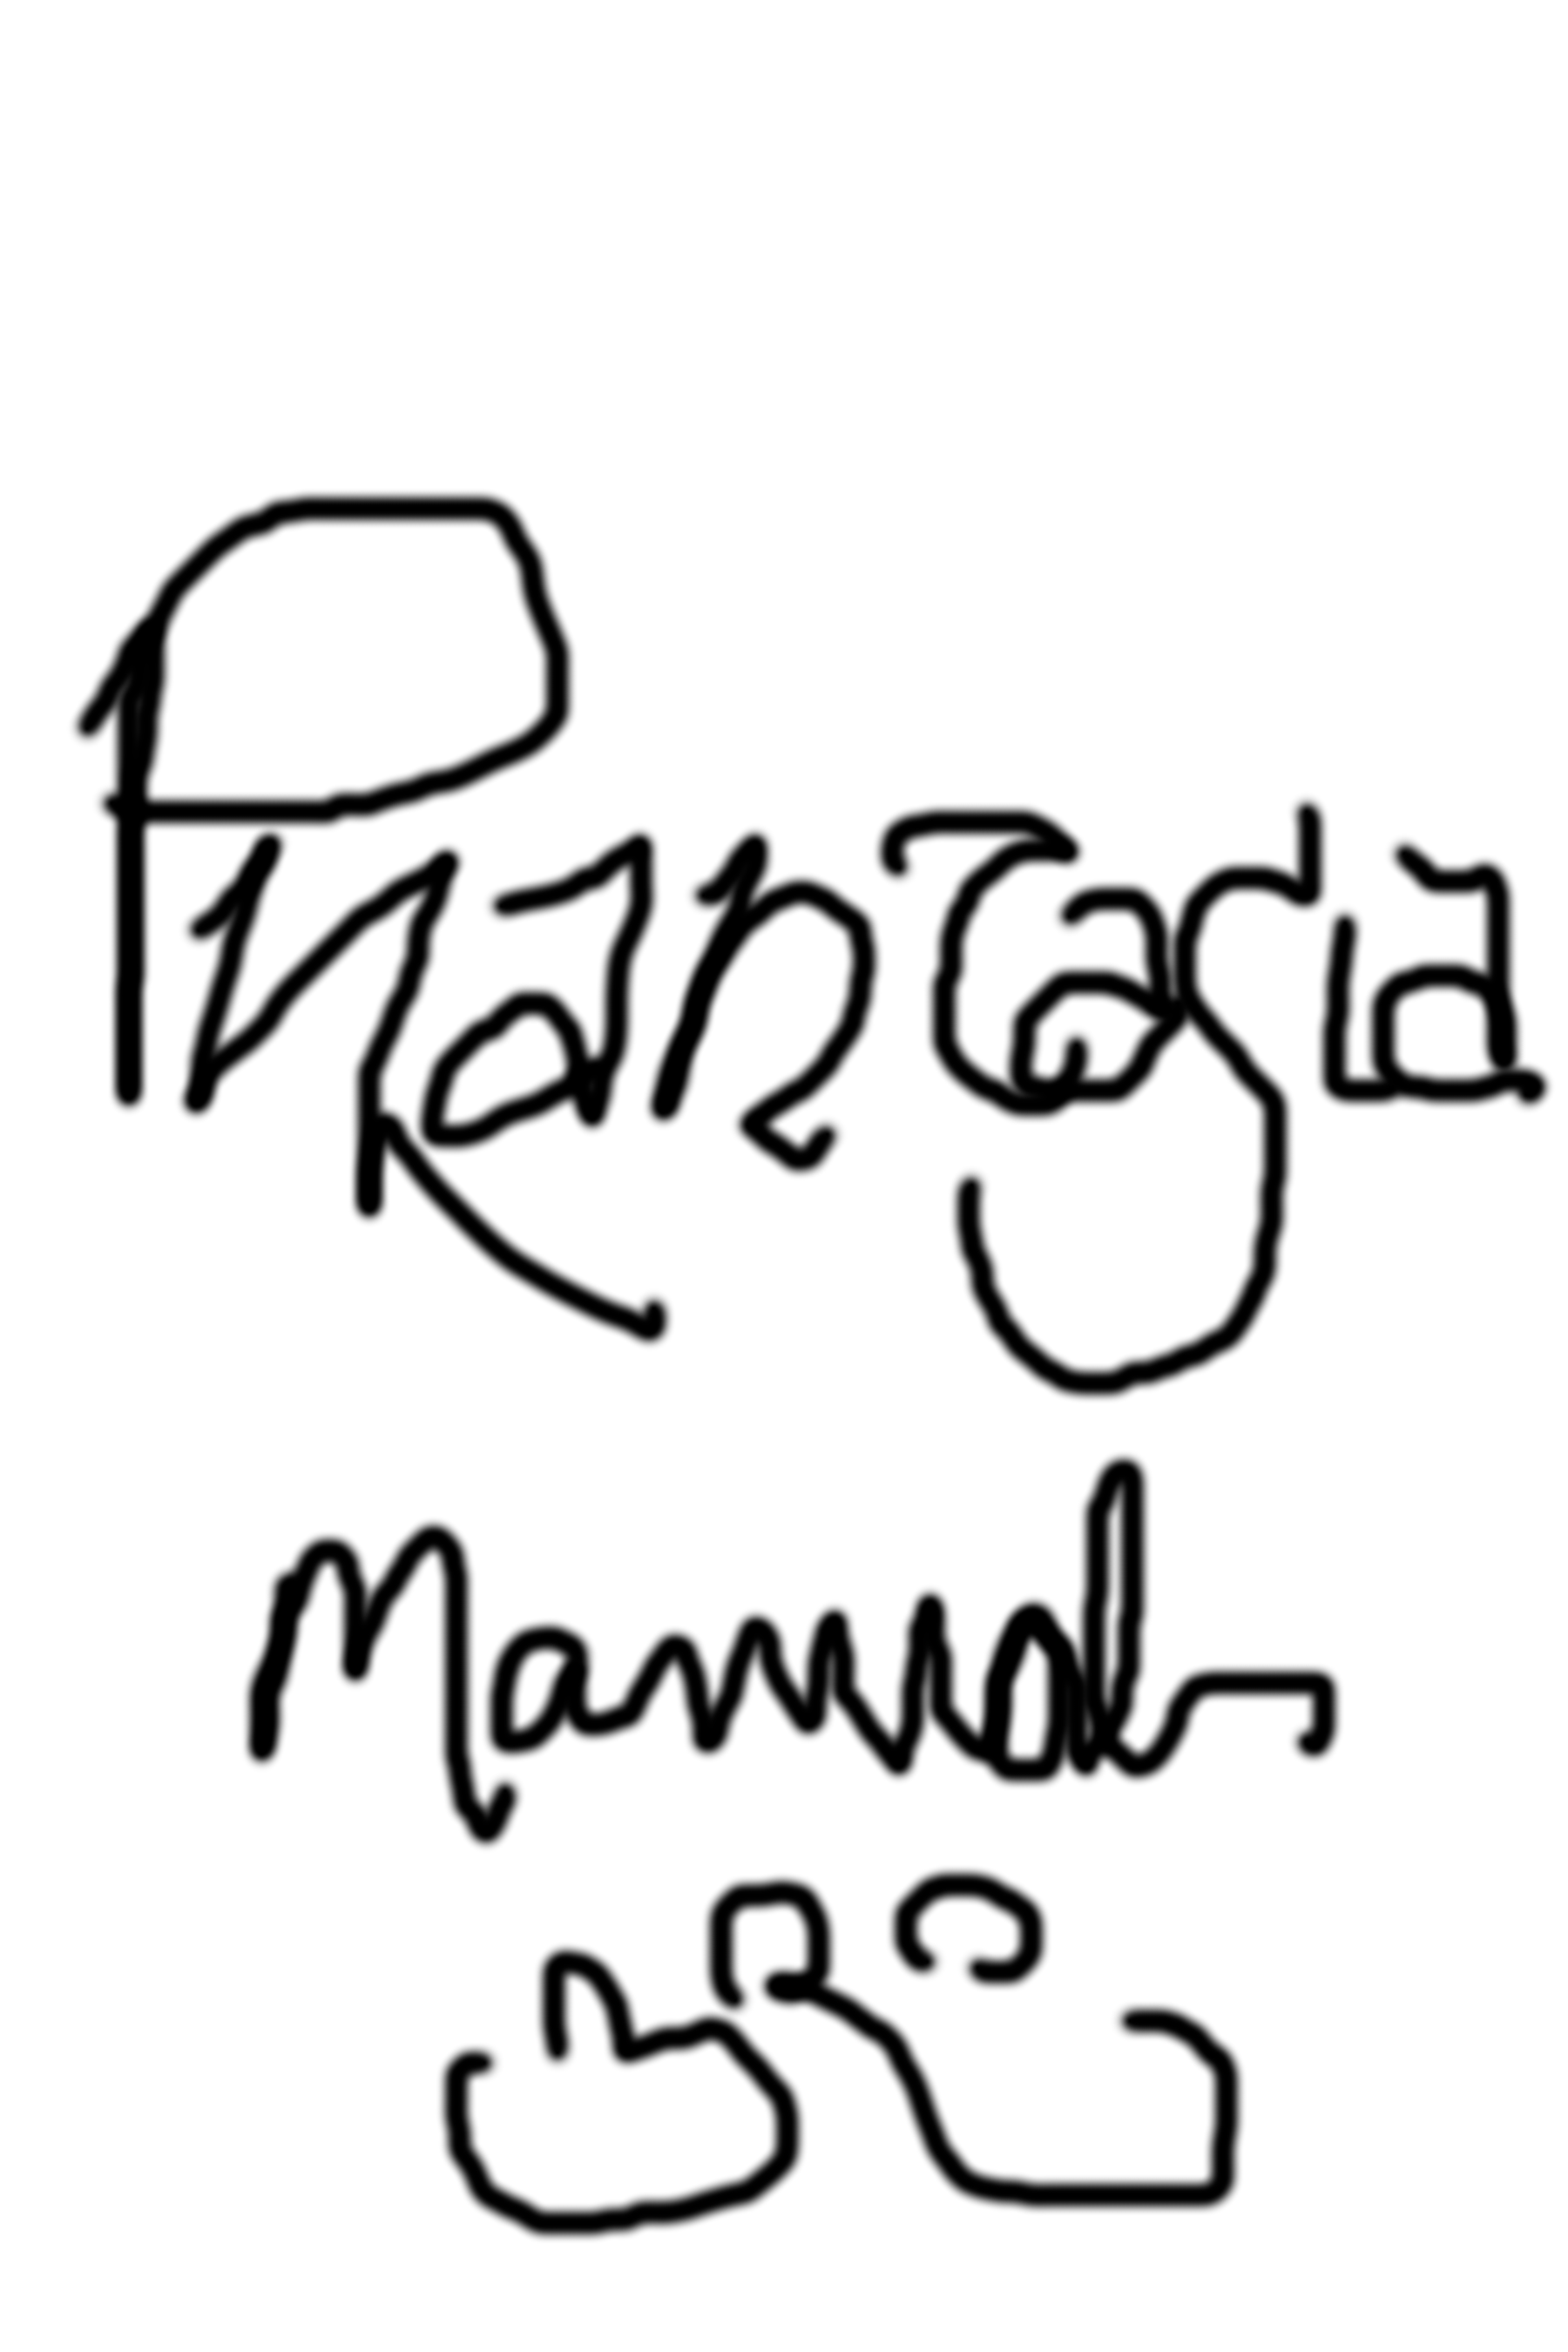
\includegraphics[interpolate,width=\paperwidth,height=\paperheight]{../Manual/Cover.png}}; 
\end{tikzpicture}


\thispagestyle{empty}

\twocolumn[

\chapter*{Introduction}\label{Introduction}

WRITEME

\bigskip

In the  \textit{Phantasia} videogame, WRITEME

\vspace{1in}\vfill

This is the \textit{Phantasia} \ifdefined\DEMO Demo \else Official \fi Player's Guide

Copyright \copyright{} 2022, Bruce-Robert Pocock

\bigskip

This  version is  for systems  in \REGION{}  using the  \TV{} television
standard. For Atari ProSystem 7800 (or Sears Tele-Games Video Arcade II)
with an optional AtariVox, MemCard, or SaveKey device.

\bigskip

This videogame software was not created, published, or licensed by Atari
or its successors.

\ifdefined\DEMO
\bigskip

This manual describes  a DEMO version of the game.  The full version may
be different.

\fi

This game has not been published in cartridge form.

\bigskip

You are hereby granted permission  to make use of the \textit{Phantasia}
videogame software for \emph{non-commercial personal use}.

Redistribution not for profit is allowed, but sales of this software
requires a license.

]

\let\cleardoublepage\clearpage

\mainmatter

\tableofcontents

\twocolumn[ \chapter{Setting Up}\label{Setting Up} ]

To play \textit{Phantasia}, you will need:

\begin{itemize}

\item An Atari console: the Atari ProSystem 7800, or Sears
  Tele-Games Video Arcade II
\item A TV or video display
\item A compatible two- or three-button joystick or gamepad (see WRITEME).

  \ifdefined\ATARIAGESAVE
\item Optional: an AtariVox device with speakers or headphones
\item The \textiit{Phantasia} game cartridge
  \else
\item Optional,  but recommended:  A memory  device: an  AtariVox device
  with  (optional)  speakers or  headphones,  or  a MemCard  or  SaveKey
  device.
\item A  multi-cart with the  \textit{Phantasia} data  on it such  as the
  \textit{Concerto} cartridge or \textit{Dragonfly}
  \fi
\end{itemize}

\begin{figure*}[b]
  \begin{center}
    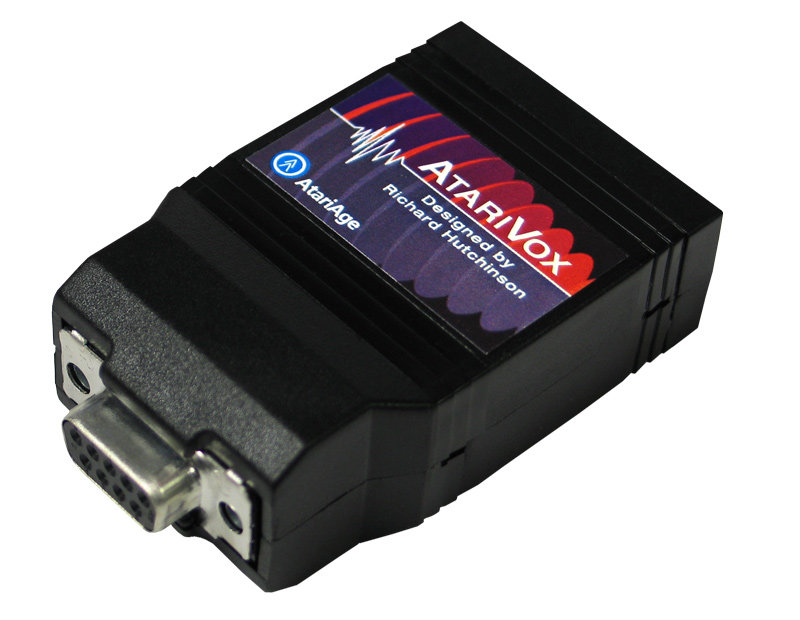
\includegraphics[width=\columnwidth]{../Manual/AtariVox.jpeg}
    \ifdefined\ATARIAGESAVE
    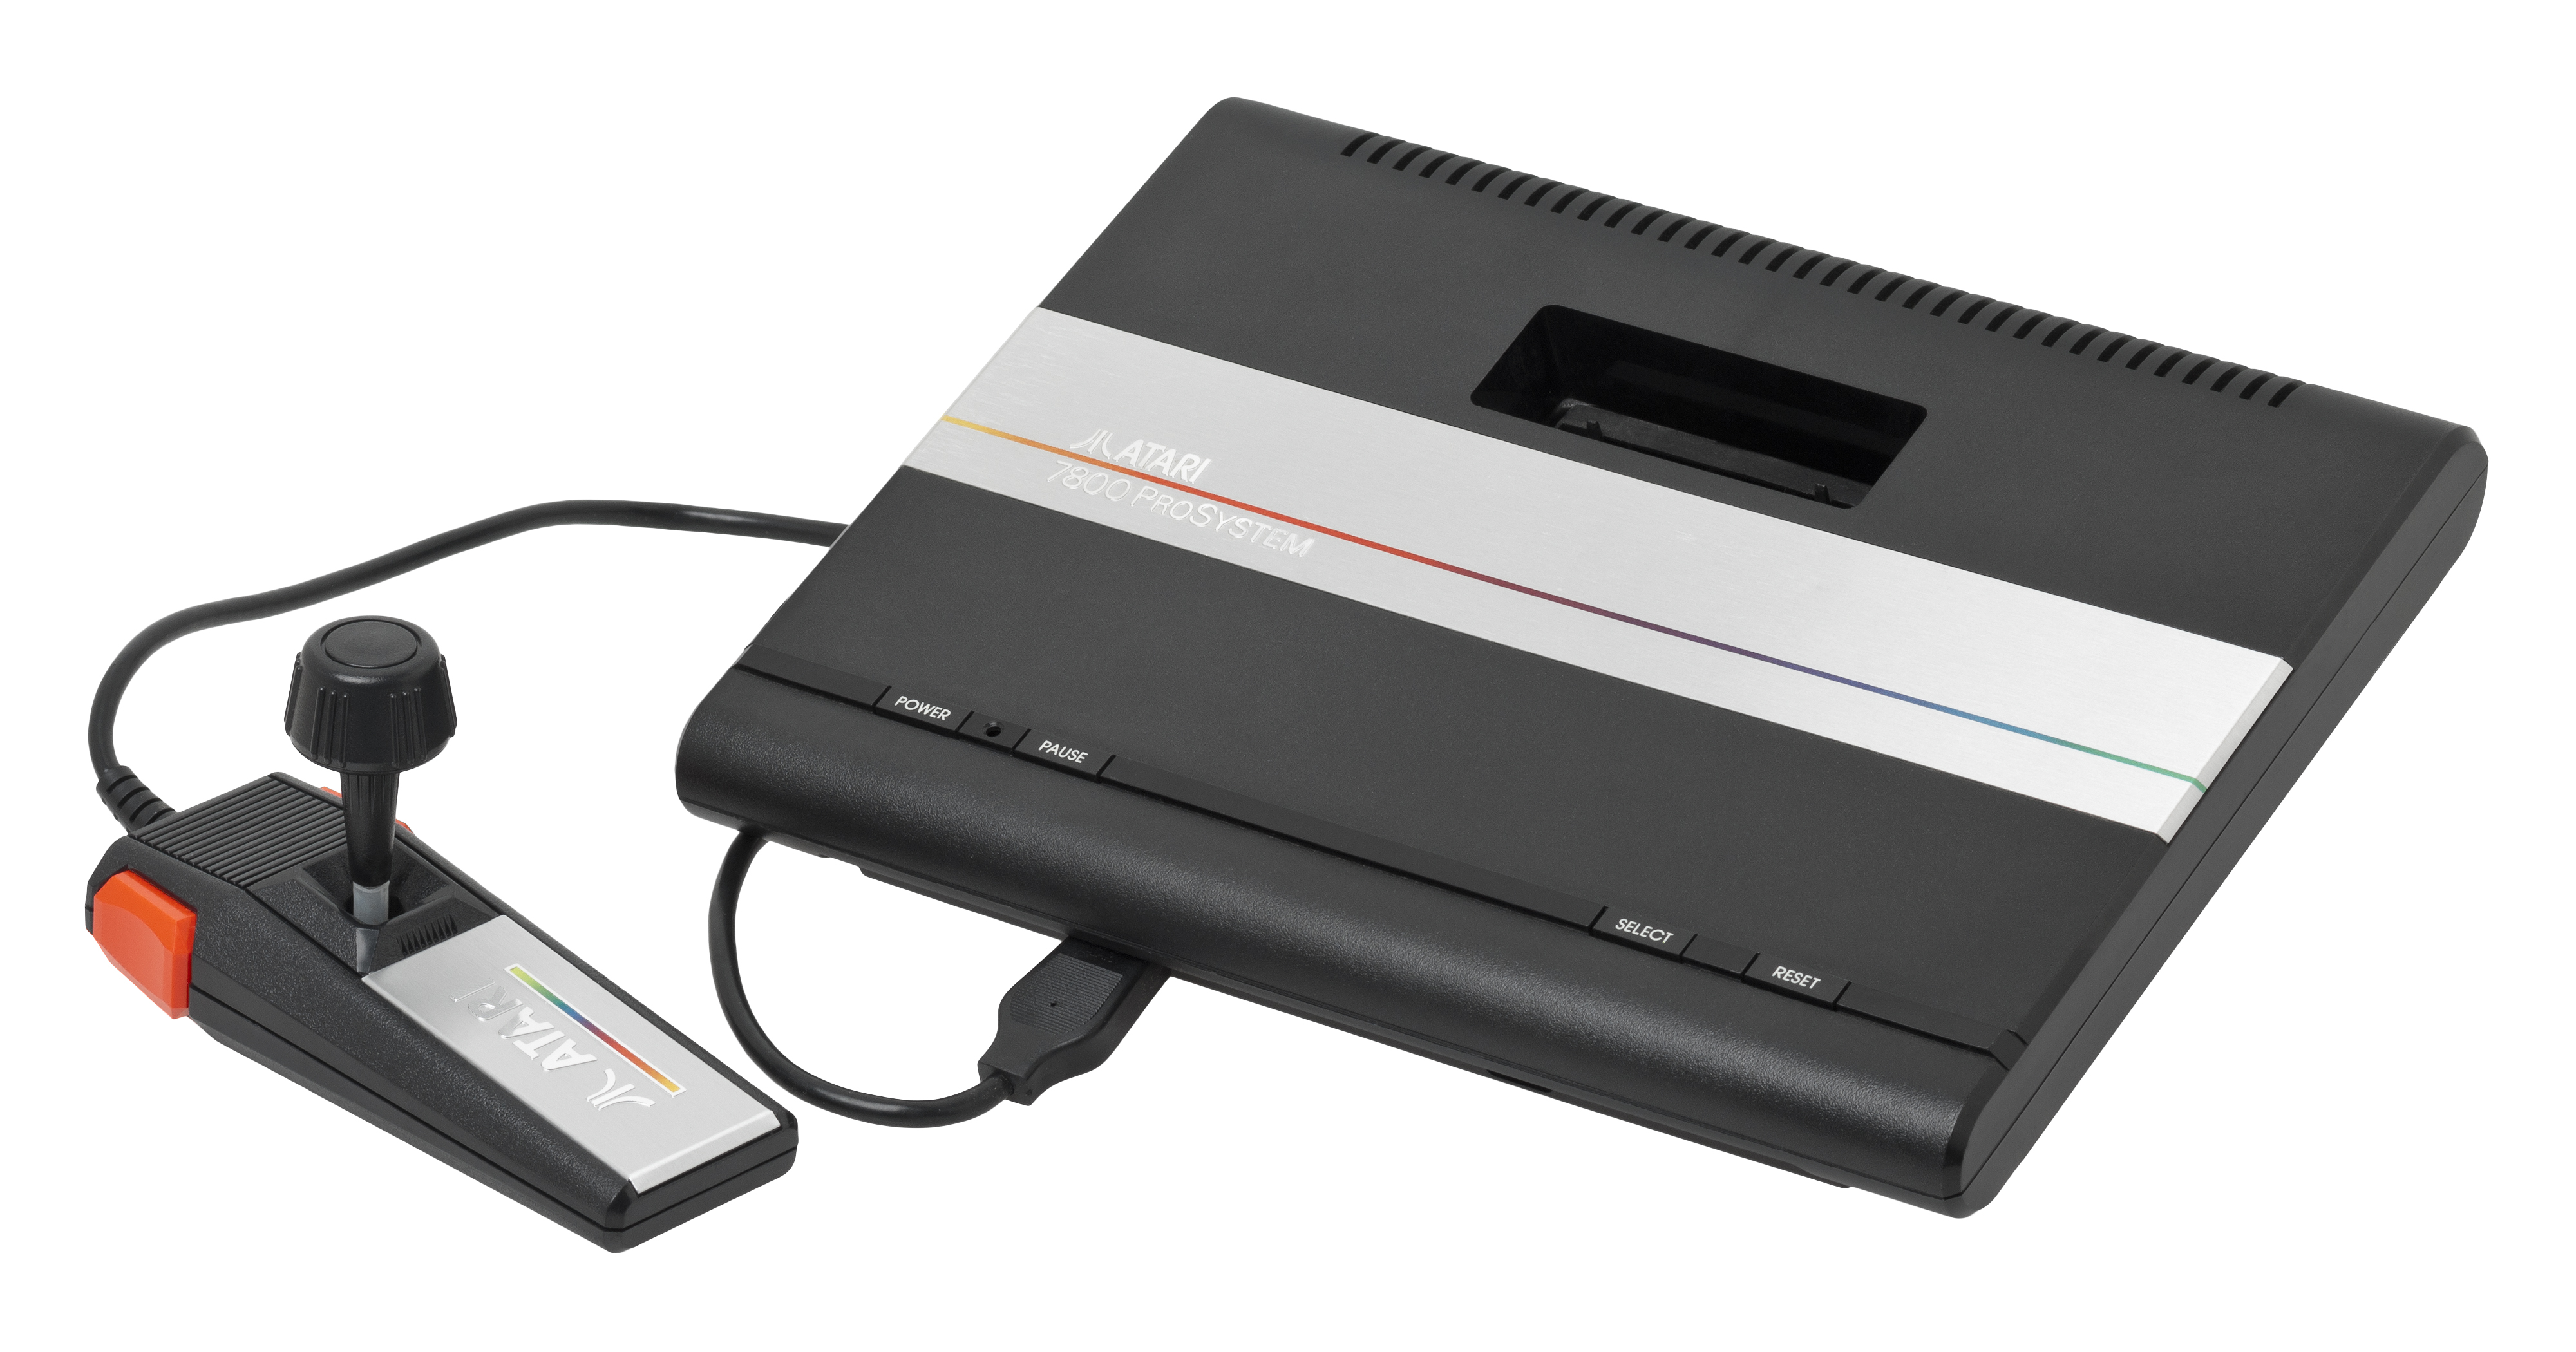
\includegraphics[width=\columnwidth]{../Manual/Atari-7800.png}
    \else
    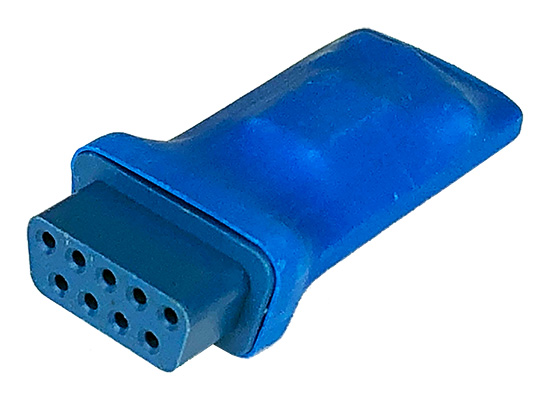
\includegraphics[width=\columnwidth]{../Manual/SaveKey.jpeg}
    \fi
  \end{center}
\end{figure*}

Set up your console with your TV or video display. Connect a joystick to
the \emph{left} controller port, and the memory
device (if any) to the \emph{right} controller port.

Finally, insert  the \textit{Phantasia}  game cartridge (with  the label
facing  up)  into  the  cartridge  slot,  and  turn  the  \textbf{Power}
\textbf{on}.

\begin{figure}[h]
  \begin{center}
    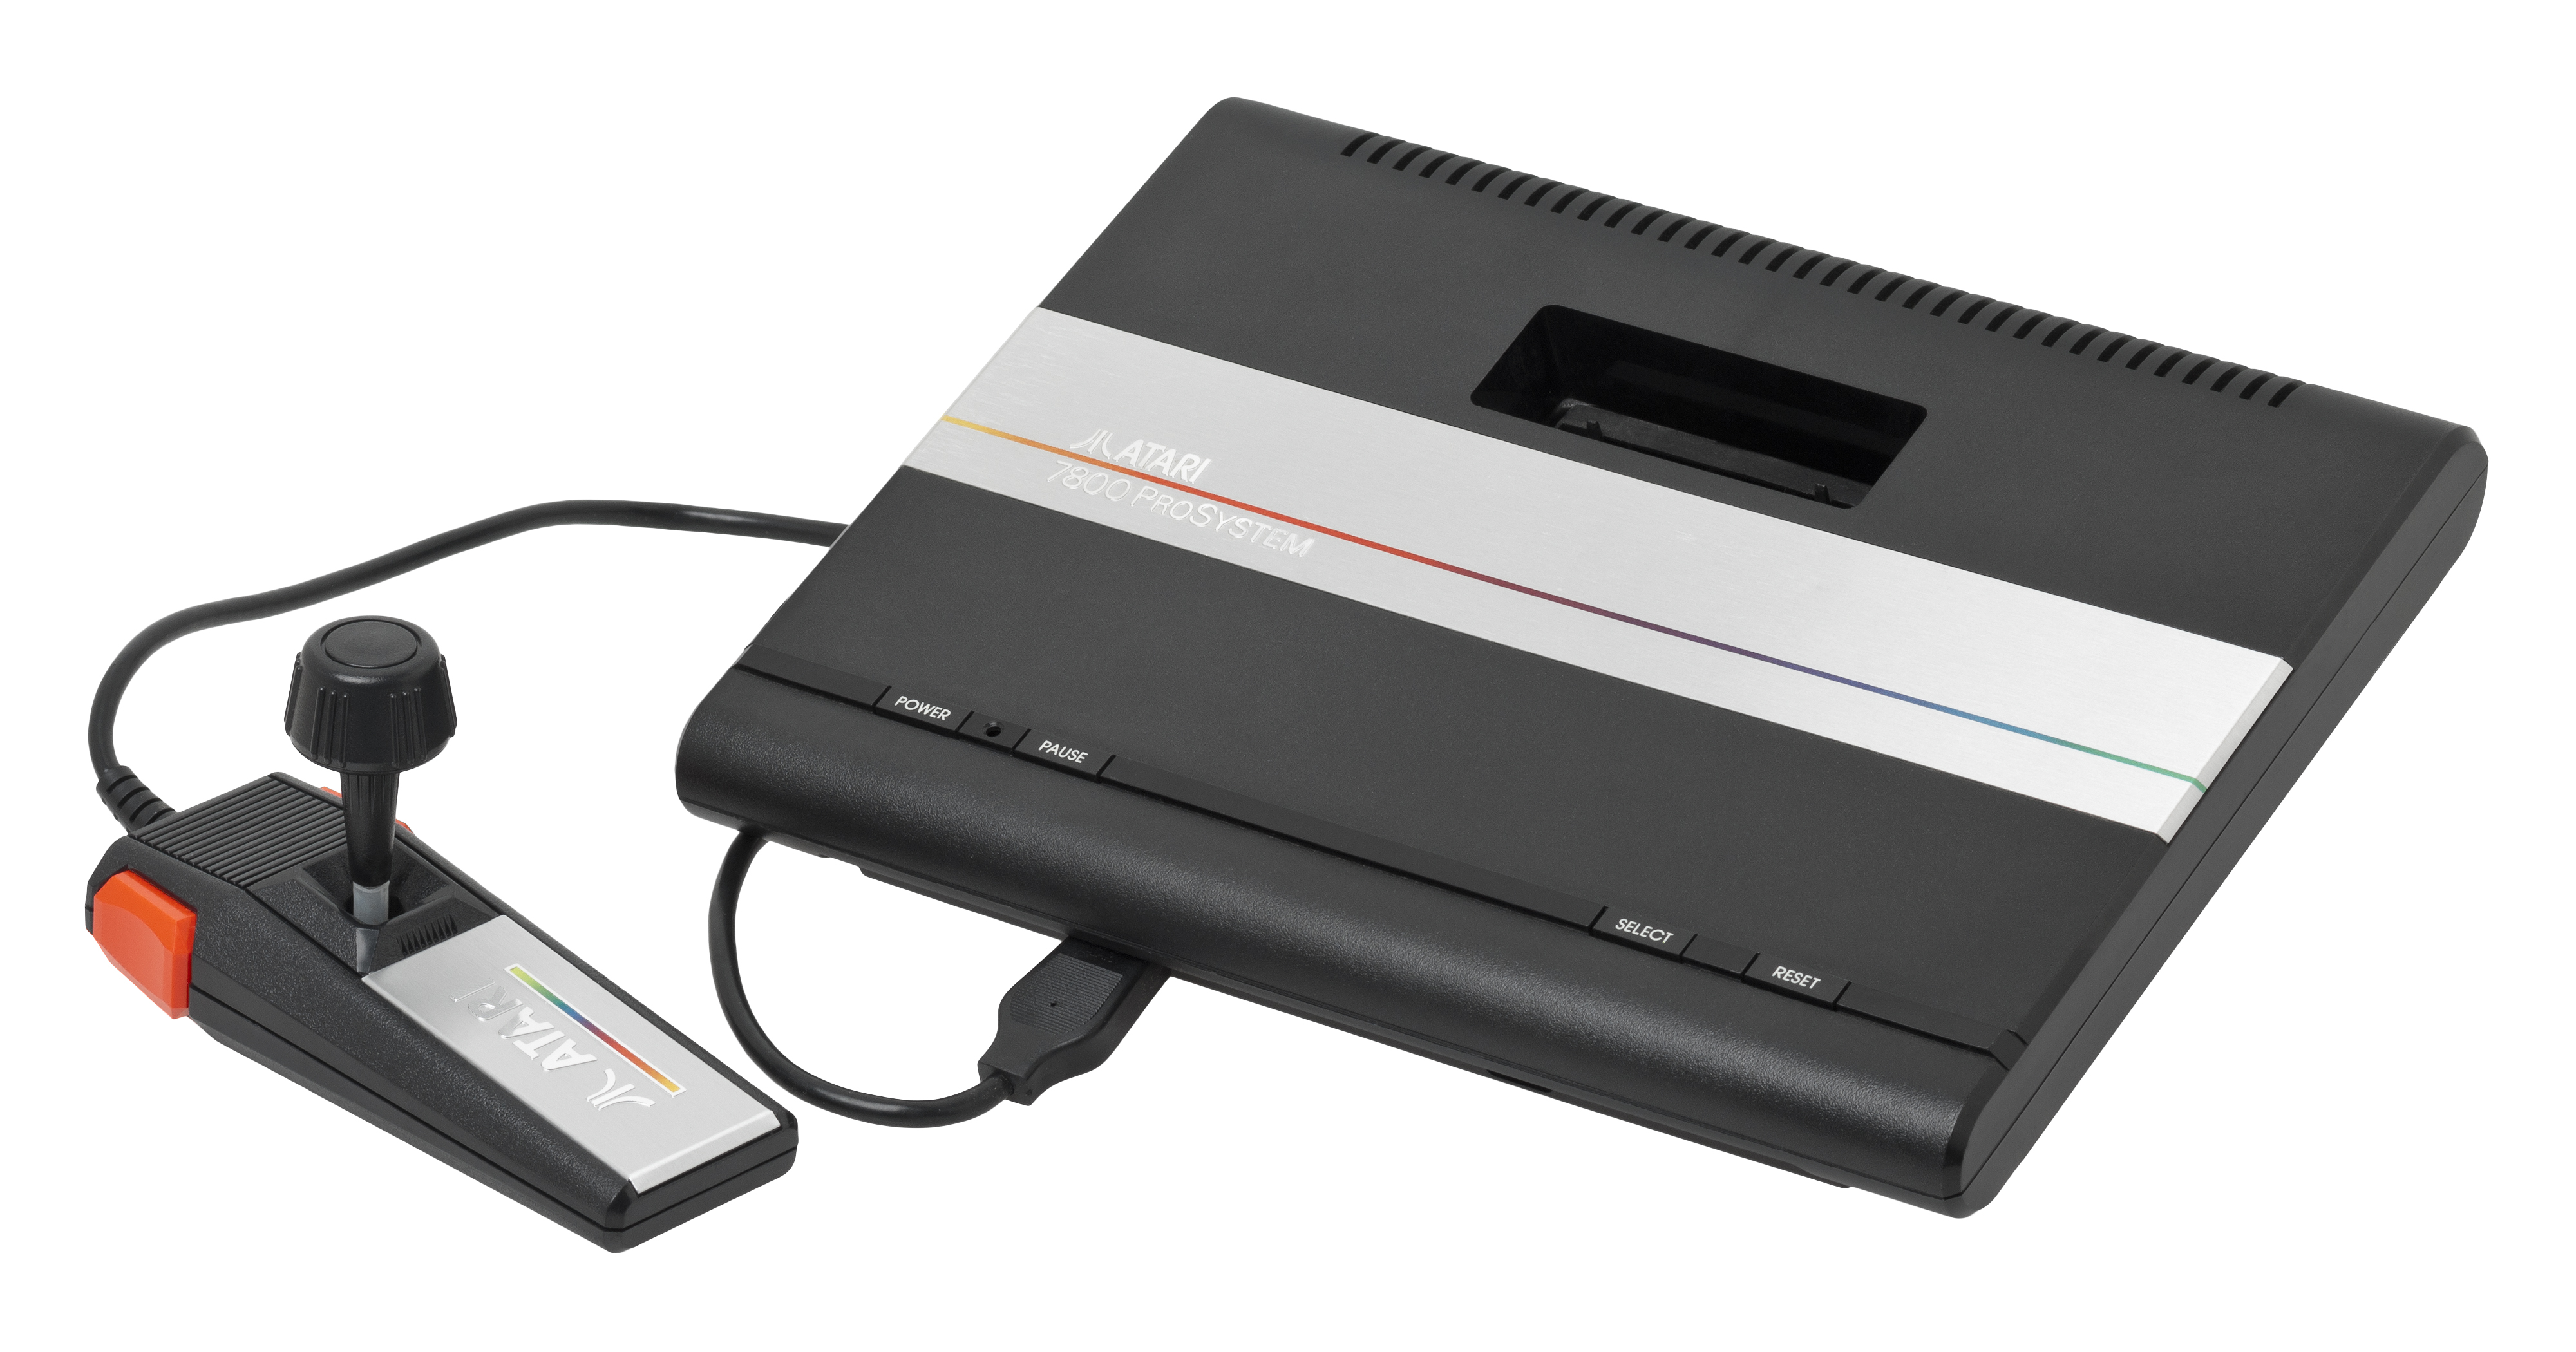
\includegraphics[width=\columnwidth]{../Manual/Atari-7800.png}
  \end{center}
\end{figure}

\section{Compatible Controllers}

There  are  three  main  kinds  of controllers  that  you  can  use  for
\textit{Phantasia}. Your  gamepad or joystick \emph{must}  be plugged in
\emph{before} you turn on the power, or it may not work correctly.

First, you can  use an Atari ProLine joystick  or compatible controller.
The left button will be button \encircle{I} and the right button will be
button \encircle{II}.

Secondly, you  can use a  SEGA \ifdefined\TVNTSC{Genesis/}\fi{}MegaDrive
gamepad  (or other  compatible controller)  may  also be  used. Use  the
\encircle{B} button as button  \encircle{I}. Use the \encircle{C} button
as  button  \encircle{II}. 

Third,  you  can  use  a  Joy2b+  controller.  Button  \encircle{I}  and
\encircle{II} will work as expected. Button \encircle{III} will work the
same as pressing the \textbf{Pause}  button on the console.

\vfill

\columnbreak
\chapter{How To Play}

\section{Console Controls}

\subsection{Pause Button}

Press the  \textbf{Pause} button (or  button \encircle{III} on  a Joy2b+
gamepad) once to pause the game, and again to resume playing.

\subsection{Select}

While you are  playing the game, you can use  the \textbf{Select} button
to access the game  menu. See ``Game Menu'', page~\pageref{sec:GameMenu}
for details.

\subsection{Reset}

While  you are  playing the  game,  press the  \textbf{Reset} button  to
access   the   Save   or   Quit    option.   See   ``Save   or   Quit'',
page~\pageref{sec:SaveOrQuit} for details.

\subsection{Difficulty Switches}

You cannot erase a game in progress from your memory device (or un-erase
it) unless both Difficulty Switches are moved to the ``right'' (Advanced
or Expert position). To protect your  game from being erased, set either
one  of   the  Difficulty   Switches  to   the  ``left''   (Beginner  or
Novice) position.

The Difficulty Switches are located between to the controller ports.

\subsubsection*{Expert Mode}

The Left Difficulty Switch adjusts the  difficulty of the game. When the
Left Difficulty  Switch is in  the ``right'' (Advanced or  Expert) position,
monsters will do more damage in  their attacks. When the Left Difficulty
Switch is in  the ``left'' (Beginner or Novice) position,  monsters will do
their normal  amount of  damage. You  will also  earn double  points for
defeating monsters while in the ``right'' position.

\section{Start a Game}

\begin{center}
  \includegraphics[width=\columnwidth]{../Manual/TitleNTSC.png}
\end{center}

Once  your console  is set  up and  everything is  connected, press  the
\textbf{Power} button. You'll  see the title screen appear.  If you have
an AtariVox device, you'll also hear the title spoken.

Press button  \encircle{II} to move to  the Select Slot screen.  If the
second button on your controller does  not seem to work, try turning the
\textbf{Power} off, make sure the controller is plugged in securely, and
then turn the \textbf{Power} back on.

\begin{center}
  \includegraphics[width=\columnwidth]{../Manual/SelectSlotNTSC.png}
\end{center}

Press the  \textbf{Select} switch or  move the  joystick up and  down to
choose   a  memory   slot\ifdefined\ATARIAGESAVE\else\footnote{Technical
  Note: The Slot  number chosen here is relative to  the three save game
  slots used by the \textit{Phantasia} game program. Each save game slot
  actually occupies ?? blocks on  your memory device.}\fi for your game.
There are three  memory slots possible. If someone has  already begun to
play \textit{Phantasia} in  a certain slot, your screen  will show their
name  and   avatar  (character).  If   a  slot  is  empty,   you'll  see
``\texttt{BEGIN}'' instead.

If you have a password, you can enter it instead by moving to the bottom
of   the  screen   to   PASSWORD  and   pressing  button   \encircle{I}.
See ``Entering a Password,'' page~\pageref{sec:EnteringAPassword}.

If someone has already \emph{won} the  game once, their name will appear
with a crown. See New Game Plus, page~\pageref{sec:NewGamePlus}.

\ifdefined\DEMO

\skip

This demo saves your progress in  the ``scratchpad'' area of your memory
device. It's possible that other  games might overwrite and destroy your
saved progress.  This is  just because  it's a demo,  and does  not have
a private area reserved for it.

\skip

\fi

When you have selected the slot you want to begin (or resume), press
button \encircle{I}.

\fi

When you first  choose to begin a  new game, you'll create  an avatar to
represent you in the world of Aclypt.

First, enter  a name for  your new avatar.  Press forward to  select the
next letter;  pull back to  select the  previous letter. Press  left and
right to move to the next or previous position. You can have up to eight
characters for your  name. After eight characters, the  cursor will turn
pink. Press  button \encircle{I} to proceed.  Press button \encircle{II}
to return to the \textbf{Select Slot} screen.

\begin{center}
  \includegraphics[width=\columnwidth]{../Manual/NameEntryNTSC.png}
\end{center}

Next, you'll  get to create  your avatar (character). Push  the joystick
forward or pull back to move between selections on the screen. Press the
button \encircle{I} button to edit a selection, then use the joystick to
make  a choice.  Press button  \encircle{I} to  confirm a  selection, or
button \encircle{II} button to abandon your change.

You can choose three attributes for your avatar.

\begin{itemize}
\item \textbf{Pronoun} Press button \encircle{I} to choose your avatar's
  gender pronoun: He, She, or They.
\item \textbf{Hair}  Press button  \encircle{I} to  choose the  color of
  your avatar's hair from among the colors shown.
\item \textbf{Skin}  Press button  \encircle{I} to  choose the  color of
  your avatar's skin from among the colors shown.
\end{itemize}


\begin{center}
  \includegraphics[width=\columnwidth]{../Manual/ConfirmNewGameNTSC.png}
\end{center}

\fi

\section{Exploring Aclypt}

You'll  begin at  your home  on the  island of  Atsirav in  the land  of
Aclypt. Refer  to the  map (back  cover of this  manual) for  some ideas
about the  geography of Aclypt. Other  characters in the game  will also
give you advice about places you can go and things you can do.

The Map screen shows your current status at the top.

\begin{itemize}
\item The item which you currently  have equipped. This is the item that
  you can use by pressing button \encircle{I}.
\item The shield (if any) which you currently have equipped.
\item The amount of gold and silver coins which you're carrying.
\item The name of the area in which you are now.
\item The amount of health that you  can have (the outline) and that you
  currently do have (the area that is filled in).
\end{itemize}

Below the status  area is the map display, where  you'll see the current
area in which you are traveling. Guide yourself using the joystick.

To interact  with objects  like doors  and people, walk  up to  them and
press button \encircle{I}.  Some items or characters may react
to you simply walking up to them, as well.

To   review  your   inventory,  statistics,   and  more,   press  button
\encircle{II}.

\begin{center}
  \includegraphics[width=\columnwidth]{../Manual/MapNTSC.png}
\end{center}

\section{Saving Your Progress}

The game is automatically saved to your memory device whenever you sleep
in your own  bed or an Inn.  You can also manually save  by pressing the
\textbf{Reset}  button  and choosing  \textbf{Save  and  Quit} from  the
pop-up menu.

You should leave your memory device connected at all times while playing
the game.

You   can   instead   use   a    password   to   save   your   progress.
Select  \textbf{Password} from  the \textbf{Reset}  menu to  obtain your
latest password.

\section{Conversations}

When you encounter  a person, they'll usually speak to  you. If you have
an AtariVox  connected, you'll hear  what they have  to say out  loud as
well.   After  you've   read  what   they   have  to   say,  press   the
button \encircle{I} button.

\begin{center}
  \includegraphics[width=\columnwidth]{../Manual/TextNTSC.png}
\end{center}

Some people will want to know what you have to say, in return. If that's
the case,  you'll be given  a choice of  possible answers to  give them.
Press forward or  back on the joystick to select  a response.

\begin{center}
  \includegraphics[width=\columnwidth]{../Manual/InquireNTSC.png}
\end{center}

If you want to  review what the person was asking,  you can press button
\encircle{II} to ask them to repeat themself instead.

When you've made your selection, press button \encircle{I} to continue.

\section{Battling Monsters}

Monsters and other enemies plague the world of Aclypt.

When you encounter monsters, you can  use your equipment such as weapons
and other gear to defeat them.

WRITEME

\section{Statistics}

\begin{center}
  \includegraphics[width=\columnwidth]{../Manual/StatsScreenshotNTSC.png}
\end{center}

Some of  your character's information  is always  visible at the  top of
the screen. To view more, press button \encircle{II}.

Across the top of the screen, you'll see:

\begin{itemize}
\item Your currently selected \textbf{equipment  item}. This is the item
  that you will use when you press button \encircle{I}.
\item Your currently selected \textbf{shield}.
\item The number of \textbf{crowns} (currency) that you have.
\item The number of \textbf{arrows} that you have.
\item The \textbf{name} of the area in which you are now.
\item Your score.
\item Your health.
\end{itemize}

When   you   press   button   \encircle{II},  you'll   also   see   your
inventory items. Press button \encircle{II}  again to return to the game
play screen.

While  viewing  your  inventory,  you  can  use  the  joystick  to  move
a selection arrow under  an item. The name of the item  at which you are
currently  pointing will  be  displayed  at the  bottom  of the  screen.

Inventory items come in a few basic kinds:

\begin{itemize}
\item  \textbf{Equipment items}  can be  equipped and  used in  the game
  world.  For  example,  a  dagger,  sword,  or  hammer  are  equipment.
  Press  button   \encircle{I}  to  equip   an  item  as   your  current
  equipment item.
\item \textbf{Shields}  can be equipped  and are effective  whenever you
  are  \emph{not} using  an equipment  item, for  example, when  you are
  standing still or walking. Press button \encircle{I} to equip a shield
  as your current  shield. Press button \encircle{I}  again to de-select
  that shield (and  use no shield).
\item  \textbf{Clothing} may  have  different  properties. Press  button
  \encircle{I} to wear a different article of clothing.
\item \textbf{Usable items} can be used  once and then vanish. A healing
  potion is  an example of a  usable item. Press button  \encircle{I} to
  immediately use a usable item.
\item \textbf{Quest  items} are items that  you hold on to,  to complete
  your missions.  Keys are an example  of a quest item.  These items are
  used automatically when  appropriate --- for example, when  you try to
  open a locked door, if you have the key, it will unlock.
\end{itemize}

\section{Scoring}

When you  defeat a monster, you'll  earn points. The number  of points
you earn  will increase as you  defeat more difficult monsters.  You can
also earn points for other some other actions you take in the game.

The score earned can be increased by:

\begin{itemize}
\item \ldots{}playing  in Expert  mode (by  setting the  Left Difficulty
  Switch to the ``right'' position)
\item \ldots{}defeating a more difficult version of a monster
\item  \ldots{}playing the  game  in  New Game  Plus  mode after  having
  defeated the final boss.
\end{itemize}

The score for  defeating a monster will be increased  to $2\times$ for any
one of these  factors, to $3\times$ for  any two of these  factors, and to
$4\times$ if all three are true.

\section{Winning the Game}

You can  win the  game by  discovering what dark  forces are  behind the
onslaught of so many monsters, and defeating them.

\subsection*{New Game Plus}\label{sec:NewGamePlus}

Once  you've won  the game,  you can  keep playing!  On the  screen that
appears when you win, press \textbf{Game  Reset} on your console to save
your winning score and create a ``new game, plus.''

On your second  time through, monsters will become more  difficult — but
also yield more points when defeated. WRITEME

\section{Game Over}

If  you fail  in  your mission,  your  game is  over.  However, you  can
continue, and it'll be just as if you'd never failed in the first place.
You'll start over from the last Inn you visited, or your own home.

\begin{center}
  \includegraphics[width=\columnwidth]{../Manual/GameOverNTSC.png}
\end{center}

\section{Starting Over}\label{Starting Your Adventure Over}

If you want to erase your progress and start again, you must:

\begin{itemize}
\item Go  to the Select Slot  screen, and press \textbf{Game  Select} or
  move  the joystick  left and  right until  you see  the slot  you want
  to erase.
\item Set both  of the Difficulty Switches on your  console to the ``right''
  (Advanced or Expert) position.
\item Pull  back on the  joystick, and \emph{while holding  the joystick
    back} press \emph{and hold} the \textbf{Fire} button.
\item If you're \emph{sure} you want to erase your game's progress, then
  \emph{without}  letting  go  of  the \textbf{Fire}  button,  push  the
  joystick  forward. \ifdefined\DEMO  Your  game record  will be  erased
  \emph{immediately}. \fi
\end{itemize}

\begin{center}
  \includegraphics[width=\columnwidth]{../Manual/EraseSlotNTSC.png}
\end{center}

Make sure  you want to  erase your game.  Press the joystick  forward or
back to make your choice, and press the \textbf{Fire} button.

\begin{center}
  \includegraphics[width=\columnwidth]{../Manual/ConfirmEraseNTSC.png}
\end{center}

The Left  Difficulty Switch is also  used to increase the  difficulty of
the  game.  After  erasing  your  progress,  you  may  return  the  Left
Difficulty  Switch  to  your  desired position.  (On  SECAM,  the  Right
Difficulty Switch is used to pause the game.)

\subsection{Protecting Your Game Record}

If either  of your Difficulty Switches  is in the ``left''  (Beginner or
Novice) position, you can't erase a game slot.

\subsection{Recovering an Erased Game}

If you have \emph{just} erased a game's progress, and no one has started
a new game using the same slot yet, you may be able to un-erase it.

To recover  an erased game,  follow the same steps  as if you  wanted to
erase  a game.  Press  left and  right  on the  joystick  to select  the
now-empty  slot  (the  screen  will say  ``\texttt{BEGIN}'').  Set  both
Difficulty Switches to the ``right'' (Advanced or Expert) position, pull
back  on  the joystick,  and  \emph{while  holding  it back},  hold  the
\textbf{Fire} button.

If your  game's progress can be  recovered, you'll see that  the slot is
\texttt{ERASED} with your name. Press  forward on the joystick. The game
will immediately become available to resume.

It is \emph{not possible} to recover  a saved game's progress once a new
game has been started in the same memory slot. If you accidentally start
a new  game, but have  not confirmed your  name yet, \emph{turn  off the
  power briefly}, then try the recovery steps above.

\chapter{Exploring Aclypt}

\chapter{Weapons and Items}

\columnbreak
\chapter{Monsters}

\columnbreak
\chapter{Troubleshooting}

\section{Sad Face Screen}

If you  see the Sad  Face screen,  the game is  trying to tell  you that
there is a problem.

From here, you can press the \textbf{Game Reset} switch to return to the
Title Screen.

The game  has encountered an  error and cannot continue.  Please contact
\href{mailto:support@star-hope.org}{support@star-hope.org}           for
additional assistance. Send the code  number that appears on this screen
with your email.

\section{No voices}

On the title  screen, you'll hear the AtariVox announce  the name of the
game. If  you don't, make  sure that the  AtariVox is connected  and the
speakers (or headphones) are connected, powered on, and turned up.

Naturally,  there are  no  voices  when playing without an AtariVox device. 

\pagebreak
\chapter{Credits}


\textit{Phantasia} was created by Bruce-Robert  Pocock. 

\bigskip


\subsection{Testers}

\vfill


\begin{center}
  
\includegraphics[width=.333\columnwidth]{../Manual/BRP.png}
\end{center}

\clearpage
\addcontentsline{toc}{chapter}{Map of Aclypt}
\thispagestyle{empty}
\begin{tikzpicture}[overlay, remember picture]
  \node[anchor=north west, xshift=-4pt, yshift=4pt] 
  at (current page.north west)
  {\includegraphics[interpolate,width=\paperwidth,height=\paperheight]{../Manual/AclyptMap.png}};
\end{tikzpicture}

\end{document}
